\section{Problem formulation}

\subsection{Multilateration}\label[secc]{trilat}
Multilateration is the process of determining the positions of unknown points in space by measurements of distances from known points \cite{trilat_website}. In order
to perform this task in two-dimensional space, at least three known points are needed.


Given $n\geq 3$ agents located at positions $\mathbf{x}_{a}\in\mathbb{R}^{2},\; 0\leq a<n$ the location 
of an entity, denoted by $\mathbf{y}\in\mathbb{R}^{2}$, can be determined as follows:
\begin{enumerate}
  \item The entity broadcasts signal and starts a timer at $t_{0}$.
  \item Agents at $\mathbf{x}_{a}$ receives broadcasted signal and immediately responds with a packet containing $\mathbf{x}_{a}$.
  \item When receiving the packet from agent ${a}$, the entity stores the time of reception in a variable $t_{1, a}$.
  \item When at least 3 agents have responded, the entity calculates the distance
  from itself to agent $a$: $d_{a} = \frac{1}{2}c(t_{1, a} - t_{0})$, where $c$ is the speed of light. The factor $\frac{1}{2}$ is due to the signal traveling
  two times the distance between the entity and agent $a$ (the ping travels from the entity to the agent, and the packet
  sent by the agent travels back again).
  \item Based on the distances, $d_{a}$, and the positions of the agents, $\mathbf{x}_{a}$, the entity can
  determine its position by calculating the point where circles centered at $\mathbf{x}_{a}$ with radii $d_{a}$ intersect.
\end{enumerate}
\figref{trilat_example} shows how the position of an entity can be determined from the known positions of 3 agents.
\begin{figure}[H]
  \centering
  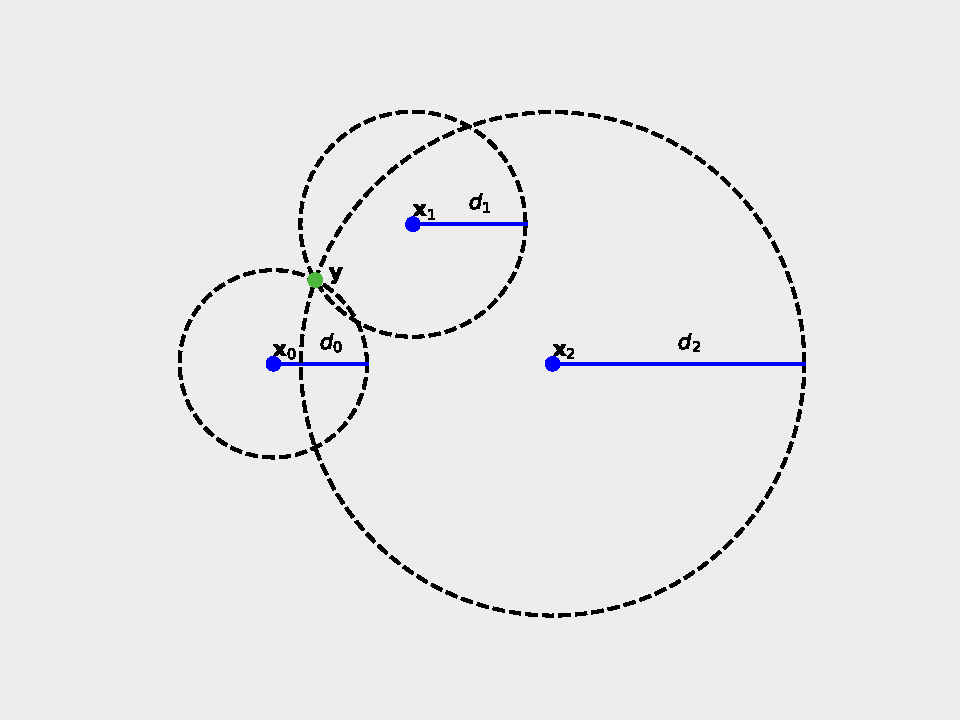
\includegraphics[width=.75\textwidth]{figs/trilateration_example.pdf}
  \caption{Position, $\mathbf{y}$, of entity determined by trilateration using known positions of $n = 3$ agents.}
  \label[fig]{trilat_example}
\end{figure}
\todo{mention how spread of agents is benefitial}

\subsection{Coverage}\label[secc]{coverage}
As the goal of the swarm is to set up a network of agents in order to deliver precise positional data to entities entering the mission space,
it is clear from the previous section that three or more agents are needed to perform the task. Hence a point $\mathbf{y}\in\mathcal{F}$ is said
to be \textit{covered} iff. it is within communication range of at least three agents.

\subsection{Objective function derivation}\label[secc]{obj_formulation}
The objective function presented here is inspired by \cite{sun2014escaping}, but differs in that for the purpose of multilateration, it is required that at least three agents must be within
range of a point in order for the point to be covered.\newline
We assume we have a total of $N$ agents in a swarm $\mathcal{N}$ at our disposal. Furthermore it is assumed that all agents have homogenous local probability with respect to $r_{a}$:
\begin{equation}\label[eq]{homogenous_r}
  \begin{split}
    r_{a} &= r\;\forall\; a\in\mathcal{N}\\
    \tilde{V}(\mathbf{x}_{a}) &= V(\mathbf{x}_{a}, r)\\
    \tilde{V}_{c}(\mathbf{x}_{a}) &= V_{c}(\mathbf{x}_{a}, r)\\
    \tilde{p}(\mathbf{x}_{a}, \mathbf{y}) &= \hat{p}(\mathbf{x}_{a}, \mathbf{y}, r)
  \end{split}
\end{equation}
The probability of a point $\mathbf{y}$ being covered by $\mathcal{N}$ can now be expressed as:
\begin{equation}\label[eq]{cover_prob}
  \Phi^{3^{+}}_{\mathcal{N}}(\mathbf{y}) = 1 - \Phi^{0}_{\mathcal{N}}(\mathbf{y}) - \Phi^{1}_{\mathcal{N}}(\mathbf{y}) - \Phi^{2}_{\mathcal{N}}(\mathbf{y})
\end{equation}
In order to formulate a distributed optimization algorithm, we rewrite the coverage supplied by $\mathcal{N}$ with focus on a single drone $a$.
We partition the swarm, $\mathcal{N}$, into two disjoint sets: $\{a\}$ and $\mathcal{N}\setminus\{a\}$. Using this we can rewrite \eqref{cover_prob} as:
\begin{equation}\label[eq]{distr_cover_derivation}
  \begin{split}
    \Phi^{3^{+}}_{\mathcal{N}}(\mathbf{y}) &= 1\\
    &- \big(1-\tilde{p}(\mathbf{x}_{a}, \mathbf{y})\big)\prod_{k\in\mathcal{N}\setminus\{a\}}\big(1-\tilde{p}(\mathbf{x}_{k}, \mathbf{y}))\\
    &- \tilde{p}(\mathbf{x}_{a}, \mathbf{y})\prod_{k\in\mathcal{N}\setminus\{a\}}\big(1-\tilde{p}(\mathbf{x}_{k}, \mathbf{y}))\\
    &- \big(1-\tilde{p}(\mathbf{x}_{a}, \mathbf{y})\big)\sum_{j\in\mathcal{N}\setminus\{a\}}\tilde{p}(\mathbf{x}_{j}, \mathbf{y})\prod_{k\in\mathcal{N}\setminus\{a\}\setminus\{j\}}\big(1-\tilde{p}(\mathbf{x}_{k}, \mathbf{y})\big)\\
    &- \tilde{p}(\mathbf{x}_{a}, \mathbf{y})\sum_{j\in \mathcal{N}\setminus\{a\}}\tilde{p}(\mathbf{x}_{j}, \mathbf{y})\prod_{k\in\mathcal{N}\setminus\{a\}\setminus\{j\}}\big(1-\tilde{p}(\mathbf{x}_{k}, \mathbf{y})\big)\\
    &- \big(1-\tilde{p}(\mathbf{x}_{a}, \mathbf{y})\big)\sum_{\mathcal{A}\in Comb(\mathcal{N}\setminus\{a\}, 2)}\prod_{j\in\mathcal{A}}\tilde{p}(\mathbf{x}_{j}, \mathbf{y})\prod_{k\in\mathcal{N}\setminus\{a\}\setminus\mathcal{A}}\big(1-\tilde{p}(\mathbf{x}_{k}, \mathbf{y})\big)\\
    &= 1\\
    &- \prod_{k\in\mathcal{N}\setminus\{a\}}\big(1-\tilde{p}(\mathbf{x}_{k}, \mathbf{y}))\\
    &- \sum_{j\in\mathcal{N}\setminus\{a\}}\tilde{p}(\mathbf{x}_{j}, \mathbf{y})\prod_{k\in\mathcal{N}\setminus\{a\}\setminus\{j\}}\big(1-\tilde{p}(\mathbf{x}_{k}, \mathbf{y})\big)\\
    &- \big(1-\tilde{p}(\mathbf{x}_{a}, \mathbf{y})\big)\sum_{\mathcal{A}\in Comb(\mathcal{N}\setminus\{a\}, 2)}\prod_{j\in\mathcal{A}}\tilde{p}(\mathbf{x}_{j}, \mathbf{y})\prod_{k\in\mathcal{N}\setminus\{a\}\setminus\mathcal{A}}\big(1-\tilde{p}(\mathbf{x}_{k}, \mathbf{y})\big)\\
  \end{split}
\end{equation}
Applying \eqref{Phi_def} to \eqref{distr_cover_derivation} yields:
\begin{equation}\label[eq]{local_coverage}
  \begin{split}
    \Phi^{3^{+}}_{\mathcal{N}}(\mathbf{y}) &= 1 - \Phi^{0}_{\mathcal{N}\setminus\{a\}}(\mathbf{y}) - \Phi^{1}_{\mathcal{N}\setminus\{a\}}(\mathbf{y}) - \Phi^{2}_{\mathcal{N}\setminus\{a\}}(\mathbf{y})\big(1-\tilde{p}(\mathbf{x}_{a}, \mathbf{y})\big)\\
    &= \Phi^{3^{+}}_{\mathcal{N}\setminus\{a\}}(\mathbf{y}) + \Phi^{2}_{\mathcal{N}\setminus\{a\}}(\mathbf{y})\tilde{p}(\mathbf{x}_{a}, \mathbf{y})\\
    &= \Phi^{3^{+}}_{\mathcal{N}\setminus\{a\}}(\mathbf{y})\big(1-\tilde{p}(\mathbf{x}_{a}, \mathbf{y})\big) + \Phi^{2+}_{\mathcal{N}\setminus\{a\}}(\mathbf{y})\tilde{p}(\mathbf{x}_{a}, \mathbf{y})\\
  \end{split}
\end{equation}
The interpretation of \eqref{local_coverage} is as follows: 
The first term gives the probability that agent $a$ is not able to communicate with an entity at $\mathbf{y}$, but at least three of the other agents are. The second term gives the probability that $a$ as well as at least two other agents are able to
communicate with an entity placed at $\mathbf{y}$.

As the goal of the swarm is to cover as large a portion of $\mathcal{F}$ as possible, and we want to do this in a distributed manner, we state the
global objective function:
\begin{equation}\label[eq]{rewritten_objective}
  \begin{split}
    H(\mathbf{x}_{\mathcal{N}}) &= \int_{\mathcal{F}}\Phi^{3^{+}}_{\mathcal{N}\setminus\{a\}}(\mathbf{y}) + \Phi^{2}_{\mathcal{N}\setminus\{a\}}(\mathbf{y})\tilde{p}(\mathbf{x}_{a}, \mathbf{y})d\mathbf{y}\\
    &= \int_{\mathcal{F}}\Phi^{3^{+}}_{\mathcal{N}\setminus\{a\}}(\mathbf{y})d\mathbf{y} + \int_{\mathcal{F}}\Phi^{2}_{\mathcal{N}\setminus\{a\}}(\mathbf{y})\tilde{p}(\mathbf{x}_{a}, \mathbf{y})d\mathbf{y}\\
  \end{split}
\end{equation}
We note that the first term in \eqref{rewritten_objective} is independent of the position of $a$ in both its domain and integrand. Thus we can rewrite the objective function as:
\begin{equation}
  H(\mathbf{x}_{\mathcal{N}}) = \tilde{H}(\mathbf{x}_{\mathcal{N}\setminus\{a\}}) + H_{a}(\mathbf{x}_{\mathcal{N}})
\end{equation}
Where the \textit{local} objective of agent $a$ is defined as:
\begin{equation}\label[eq]{local_objective}
  H_{a}(\mathbf{x}_{\mathcal{N}}) = \int_{\mathcal{F}}\Phi^{2}_{\mathcal{N}\setminus\{a\}}(\mathbf{y})\tilde{p}(\mathbf{x}_{a}, \mathbf{y})d\mathbf{y}
\end{equation}

As in \cite{sun2014escaping} we note that from the viewpoint of agent $a$, the swarm can be partitioned into three disjoint sets: $\{a\}$, $\mathcal{B}_{a}$ and $\mathcal{C}_{a}$. The latter sets are defined as:
\begin{subequations}\label[eq]{neigh_def}
  \begin{equation}
    \mathcal{B}_{a} = \{j\in\mathcal{N}\setminus\{a\}: \norm{\mathbf{x}_{a}-\mathbf{x}_{j}} \leq r\}
  \end{equation}
  \begin{equation}
    \mathcal{C}_{a} = \{j\in\mathcal{N}\setminus\{a\}: \norm{\mathbf{x}_{a}-\mathbf{x}_{j}} > r\}
  \end{equation}  
\end{subequations}
The set $\mathcal{B}_{a}$, from now on called the neighbours of $a$, contains all agents in the swarm, $\mathcal{N}$, whose communication disks form a non-empty intersection with that of $a$.
$\mathcal{C}_{a}$ contains all agents whose communication disks do not intersect with that of $a$.

Applying \eqref{neigh_def} to \eqref{local_objective} yields:
\begin{equation}
  \begin{split}
    H_{a}(\mathbf{x}_{\mathcal{N}}) &= \int_{\mathcal{F}}\Phi^{2}_{\mathcal{N}\setminus\{a\}}(\mathbf{y})\tilde{p}(\mathbf{x}_{a}, \mathbf{y})d\mathbf{y}\\
    &= \int_{\mathcal{F}}\Big(\Phi^{2}_{\mathcal{B}_{a}}(\mathbf{y}) + \Phi^{2}_{\mathcal{C}_{a}}(\mathbf{y}) + \Phi^{1}_{\mathcal{B}_{a}}(\mathbf{y})\Phi^{1}_{\mathcal{C}_{a}}(\mathbf{y})\Big)\tilde{p}(\mathbf{x}_{a}, \mathbf{y})d\mathbf{y}
  \end{split}
\end{equation}
Partitioning the domain of integration into the visible set and invisible set of agent $a$, and noting that $\tilde{p}(\mathbf{x}_{j}, \mathbf{y}) = 0\;\forall\;j\in\mathcal{C}_{a},\;\mathbf{y}\in\tilde{V}(\mathbf{x}_{a})$ such that
$\Phi^{n}_{\mathcal{C}_{a}}(\mathbf{y}) = 0\;\forall\;n\in\mathbb{Z}^{+},\;\mathbf{y}\in\tilde{V}(\mathbf{x}_{a})$, and $\tilde{p}(\mathbf{x}_{a}, \mathbf{y}) = 0\;\forall\;\mathbf{y}\in\tilde{V}_{c}(\mathbf{x}_{a})$ yields:
\begin{equation}\label[eq]{local_objective_derivated}
  \begin{split}
    H_{a}(\mathbf{x}_{\mathcal{N}}) &= \int_{\tilde{V}(\mathbf{x}_{a})}\Big(\Phi^{2}_{\mathcal{B}_{a}}(\mathbf{y}) + \Phi^{2}_{\mathcal{C}_{a}}(\mathbf{y}) + \Phi^{1}_{\mathcal{B}_{a}}(\mathbf{y})\Phi^{1}_{\mathcal{C}_{a}}(\mathbf{y})\Big)\tilde{p}(\mathbf{x}_{a}, \mathbf{y})d\mathbf{y}\\
    &+ \int_{\tilde{V}_{c}(\mathbf{x}_{a})}\Big(\Phi^{2}_{\mathcal{B}_{a}}(\mathbf{y}) + \Phi^{2}_{\mathcal{C}_{a}}(\mathbf{y}) + \Phi^{1}_{\mathcal{B}_{a}}(\mathbf{y})\Phi^{1}_{\mathcal{C}_{a}}(\mathbf{y})\Big)\tilde{p}(\mathbf{x}_{a}, \mathbf{y})d\mathbf{y}\\
    &= \int_{\tilde{V}(\mathbf{x}_{a})}\Phi^{2}_{\mathcal{B}_{a}}(\mathbf{y})p(\norm{\mathbf{x}_{a}-\mathbf{y}})d\mathbf{y} = \tilde{H}_{a}(\mathbf{x}_{\{a\}\cup\mathcal{B}_{a}})
  \end{split}
\end{equation}
Using \eqref{local_objective_derivated} the global objective function can be written as:
\begin{equation}
  H(\mathbf{x}_{\mathcal{N}}) = \int_{\tilde{V}(\mathbf{x}_{a})}\Phi^{2}_{\mathcal{B}_{a}}(\mathbf{y})p(\norm{\mathbf{x}_{a}-\mathbf{y}})d\mathbf{y} + \int_{\mathcal{F}}\Phi^{3+}_{\mathcal{N}\setminus\{a\}}(\mathbf{y})d\mathbf{y}
\end{equation}
where the first term is the local objective function of agent $a$ which depends only on the position of $a$ (in both domain and integrand) and the positions of the neighbours of $a$. The second term does not depend on the position of $a$.

\subsection{Optimization problem formulation}
An optimal coverage has to fulfill two demands: The largest possible portion of $\mathcal{F}$ must the within range of at least three agents, and agents must be positioned within the feasible space. Thus for any agent $a$,
we want it to position itself such that it makes the largest possible contribution towards the global objective. Using \eqref{local_objective_derivated} we state the distributed optimal coverage problem as:
\begin{equation}
  \max_{\mathbf{x}_{a}} H(\mathbf{x}_{\mathcal{N}}) = \max_{\mathbf{x}_{a}} \tilde{H}_{a}(\mathbf{x}_{\{a\}\cup\mathcal{B}_{a}}) = \max_{\mathbf{x}_{a}} \int_{\tilde{V}(\mathbf{x}_{a})}\Phi^{2}_{\mathcal{B}_{a}}(\mathbf{y})p(\norm{\mathbf{x}_{a}-\mathbf{y}})d\mathbf{y}\quad\mathrm{s.t.}\;\mathbf{x}_{a}\in\mathcal{F}
\end{equation}